\chapter{更多电路专题}

在前面我们已经学习了所有电路原理。在这一章中我们以电路功能分类,介绍一些常用的电路模块。

\section{递次电路}\label{sec2}
在\autoref{sec35}中我们已经介绍了传统递次电路的原理,这里我们来看一下各式各样的递次电路。

\subsection{传统递次电路}
“传统”递次电路即为在多个故障逻辑门中简单循环的电路。我们在后面的推广递次和多级递次中可以看到递次电路的其他思路。

\begin{figure}[!ht]
    \centering
	\subfloat[传统递次]{\label{fig52}
\includegraphics{images/72.png}\qquad
\includegraphics{images/73.png}}
	\qquad
	\subfloat[带复位的传统递次]{\label{fig53}
\includegraphics{images/106.png}\qquad
\includegraphics{images/107.png}}
	\qquad
    \subfloat[斜式传统递次]{\label{fig54}
\includegraphics{images/78.png}\qquad
\includegraphics{images/79.png}}
	\qquad
	\subfloat[密排传统递次]{\label{fig55}
\includegraphics{images/82.png}\qquad
\includegraphics{images/83.png}}
	\qquad
	\subfloat[密排带复位传统递次]{\label{fig56}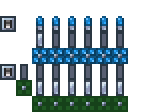
\includegraphics{images/317.png}\qquad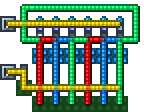
\includegraphics{images/318.png}}
	\caption{常用的传统递次电路}
\end{figure}

\autoref{fig52}和\autoref{fig53}就是我们在\autoref{sec35}中已经学习的基础电路。\autoref{fig53}是我们在\autoref{sec36}中使用到的模块。\autoref{fig55}耗尽了电线颜色,所以实际应用时需要谨慎选择。

\autoref{fig56}的复位部分使用了\nameref{sec37}。

\subsection{传统双向递次电路}\label{sec3}
双向递次电路就是可以正反两个方向循环的递次电路。正反分别用两根线控制。

\begin{figure}[!ht]
    \centering
    \subfloat[传统双向递次]{
\includegraphics{images/263.png}\qquad
\includegraphics{images/264.png}}
	\qquad
    \subfloat[密排传统双向递次]{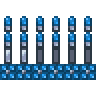
\includegraphics{images/261.png}\qquad
\includegraphics{images/262.png}}
	\qquad
    \subfloat[带复位的传统双向递次]{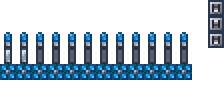
\includegraphics{images/265.png}\qquad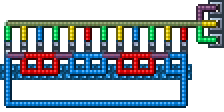
\includegraphics{images/266.png}}
	\caption{传统双向递次电路}
\end{figure}

\subsection{推广递次电路}
递次电路能形成循环,是靠的故障逻辑门改变逻辑灯状态,而逻辑灯状态又能反过来决定故障逻辑门是否激活。换言之,每一步中电路的状态都可以决定下一步的状态。这样依次下去,就形成了一个状态链。我们有理由相信,在某些特定的接线方式下,状态链会形成循环。

\begin{example}
分析如\autoref{fig59}所示的4-传统递次电路。
\begin{figure}[!ht]
\centering

\includegraphics{images/416.png}
\caption{}\label{fig59}
\end{figure}
\end{example}
\begin{solution}
4-传统递次总共有16种状态,它们对应的后继如\autoref{tab14}所示。
\begin{table}[!ht]
\centering
\begin{tabular}{|c|c|}
\hline
当前状态&下一状态\\\hline
0000&0000\\\hline
0001&1000\\\hline
0010&0001\\\hline
0011&1001\\\hline
0100&0010\\\hline
0101&1010\\\hline
0110&0011\\\hline
0111&1011\\\hline
1000&0100\\\hline
1001&1100\\\hline
1010&0101\\\hline
1011&1101\\\hline
1100&0110\\\hline
1101&1110\\\hline
1110&0111\\\hline
1111&1111\\\hline
\end{tabular}
\caption{}\label{tab14}
\end{table}

根据\autoref{tab14},我们得出4-传统递次的所有循环:
\begin{align*}
0000&\to 0000\\
1000&\to 0100\to 0010\to 0001\to 1000\\
0110&\to 0011\to 1001\to 1100\to 0110\\
0101&\to 1010\to 0101\\
0111&\to 1011\to 1101\to 1110\to 0111\\
1111&\to 1111
\end{align*}
4-传统递次一共有6个循环,其中2个1循环、1个2循环、3个4循环。
\end{solution}

\begin{example}
分析如\autoref{fig57}所示的推广递次电路。
\begin{figure}[!ht]
\centering

\includegraphics{images/426.png}
\caption{}\label{fig57}
\end{figure}
\end{example}
\begin{solution}
\begin{table}[!ht]
\centering
\begin{tabular}{|c|c|}
\hline
当前状态&下一状态\\\hline
0000&0000\\\hline
0001&1000\\\hline
0010&0001\\\hline
0011&1001\\\hline
0100&0010\\\hline
0101&1010\\\hline
0110&0011\\\hline
0111&1011\\\hline
1000&0110\\\hline
1001&1110\\\hline
1010&0111\\\hline
1011&1111\\\hline
1100&0100\\\hline
1101&1100\\\hline
1110&0101\\\hline
1111&1101\\\hline
\end{tabular}
\caption{}\label{tab15}
\end{table}
根据\autoref{tab15},我们得出该推广递次的所有循环:
\begin{align*}
0000\to &0000\\
0001\to &1000\to 0110\to 0011\to 1001\to 1110\to 0101\to 1010\to \\
        &0111\to 1011\to 1111\to 1101\to 1100\to 0100\to 0010\to 0001
\end{align*}
该推广递次一共有2个循环,其中1个1循环、1个15循环。
\end{solution}

不难看出,无论推广递次如何连接,$0000\to 0000$的1循环是不会变的,我们把这个循环叫做\textbf{平凡循环}并在之后的讨论中忽略它。如果一个推广递次的所有非零状态共同构成了一个循环,那么我们把这个循环叫做\textbf{全循环}。推广递次连接的多样化、状态的多样化、循环的多样化带来了更多的可能性。

\begin{example}
分析\autoref{fig58}中的降频电路。
\begin{figure}[!ht]
\centering

\includegraphics{images/332.png}
\caption{}\label{fig58}
\end{figure}
\end{example}
\begin{solution}
该电路分为两部分:左边两个门为2-推广递次电路,右边一个门为2-降频电路,2-推广递次的绿线接到2-降频电路的输入。

分析推广递次的输出时,不光要分析各个灯的状态,还要分析各根线的状态。本例中2-推广递次的两个灯与两根线的状态如\autoref{tab16}所示,其中两根线的初始状态设为0。

\begin{table}
\centering
\begin{tabular}{|c|c|c|c|}
\hline
状态编号&两灯状态&蓝线状态&绿线状态\\\hline
0&10&0&0\\\hline
1&01&1&0\\\hline
2&11&0&1\\\hline
\end{tabular}
\caption{}\label{tab16}
\end{table}

这个推广递次的循环为3,而且每个循环中绿线激活两次,通过2-降频电路后,每个循环中火把被激活一次。所以\autoref{fig58}中的降频电路是3-降频电路。

如果使用3-传统递次电路实现降频,因为摆线的原因,电路的宽或高至少要增加一格。推广递次在这种简单功能上有体积的优势。

如果去掉最右边的2-降频电路,左边的2-推广递次就会变成一个不均匀降频电路,或者说,(1,2)-降频电路,即周期在1与2切换。改变推广递次的门数与接线就可以得到各种各样的不均匀降频电路。串联不均匀降频电路可以得到输出更复杂的不均匀降频电路,例如串联两个(1,2)-降频电路,可以得到(1,3,2,3)-降频电路,其推导过程留给读者。

\end{solution}

并非所有推广递次都可以产生非平凡循环。

\begin{example}
\autoref{fig60}所示推广递次的状态链见\autoref{fig61}。这个状态链是一棵树,不包含任何一个非平凡循环。
\begin{figure}[!ht]
\centering

\includegraphics{images/414.png}
\caption{}\label{fig60}
\end{figure}
\begin{figure}[!ht]
\centering
\begin{forest} for tree={edge={<-},grow=west},
	[0000,name=s
		[0001
			[0010
				[0100
					[1000]
					[1001]]
				[0101
					[1010]
					[1011]]]
			[0011
				[0110
					[1100]
					[1101]]
				[0111
					[1110]
					[1111]]]]]
	\draw[->] (s) to[out=45,in=-45,looseness=3] (s);
\end{forest}
\caption{}\label{fig61}
\end{figure}
\end{example}

\begin{example}
\autoref{fig62}所示推广递次的状态链见\autoref{fig63}。这个状态链由两棵树组成。
\begin{figure}[!ht]
\centering

\includegraphics{images/415.png}
\caption{}\label{fig62}
\end{figure}
\begin{figure}[!ht]
\centering
\begin{forest} for tree={edge={<-},grow=west},
	[0000,name=s
		[0001
			[0010
				[0100]
				[0101]]
			[0011
				[0110]
				[0111]]]]
	\draw[->] (s) to[out=45,in=-45,looseness=3] (s);
\end{forest}
\quad
\begin{forest} for tree={edge={<-},grow=east},
	[1111,name=s
		[1110
			[1101
				[1011]
				[1010]]
			[1100
				[1001]
				[1000]]]]
	\draw[->] (s) to[out=135,in=-135,looseness=3] (s);
\end{forest}
\caption{}\label{fig63}
\end{figure}

\end{example}

\begin{example}
\autoref{fig65}所示推广递次的状态链见\autoref{fig64},其中既有环结构也有树结构。
\begin{figure}[!ht]
\centering

\includegraphics{images/427.png}
\caption{}\label{fig65}
\end{figure}
\begin{figure}[!ht]
\centering
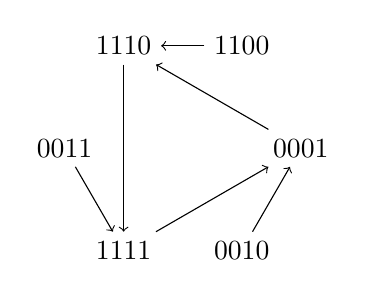
\begin{tikzpicture}
\newdimen\R
\R=1.5cm;
\node (s1) at (0:\R) {0001};
\node (se) at (120:\R) {1110};
\node (sf) at (240:\R) {1111};
\node (s2) at (300:\R) {0010};
\node (s3) at (180:\R) {0011};
\node (sc) at (60:\R) {1100};
\path [->]
    (s1) edge (se)
    (se) edge (sf)
    (sf) edge (s1)
    (s2) edge (s1)
    (s3) edge (sf)
    (sc) edge (se);
\end{tikzpicture}
\quad
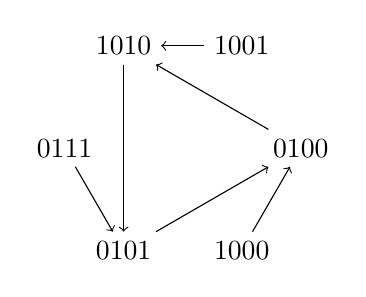
\begin{tikzpicture}
\newdimen\R
\R=1.5cm;
\node (s1) at (0:\R) {0100};
\node (se) at (120:\R) {1010};
\node (sf) at (240:\R) {0101};
\node (s2) at (300:\R) {1000};
\node (s3) at (180:\R) {0111};
\node (sc) at (60:\R) {1001};
\path [->]
    (s1) edge (se)
    (se) edge (sf)
    (sf) edge (s1)
    (s2) edge (s1)
    (s3) edge (sf)
    (sc) edge (se);
\end{tikzpicture}
\quad
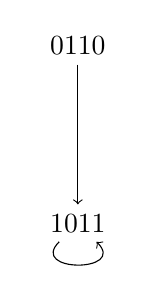
\begin{tikzpicture}
\newdimen\R
\R=1.3cm;
\node (se) at (120:\R) {0110};
\node (sf) at (240:\R) {1011};
\path [->] (se) edge (sf);
\draw [->] (sf) to[out=-135,in=-45,looseness=3] (sf);
\end{tikzpicture}
\quad
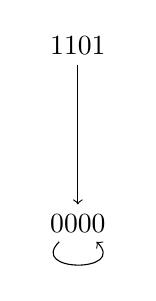
\begin{tikzpicture}
\newdimen\R
\R=1.3cm;
\node (se) at (120:\R) {1101};
\node (sf) at (240:\R) {0000};
\path [->] (se) edge (sf);
\draw [->] (sf) to[out=-135,in=-45,looseness=3] (sf);
\end{tikzpicture}
\caption{}\label{fig64}
\end{figure}
\end{example}

目前除了暴力穷举之外尚无法预测推广递次的行为,设计推广递次靠尝试与经验。

\section{驱动}

\subsection{自定义半砖驱动}
使用假人驱动可以得到60Hz的驱动。如果要进行降频,除了使用降频技术以外,还可以修改半砖装置(\autoref{i235:236})。

\begin{figure}[!ht]
\begin{center}
\subfloat[]{
\label{i235}

\includegraphics{images/235.png}
}
\qquad
\subfloat[]{
\label{i236}

\includegraphics{images/236.png}
}
\end{center}
\caption{\protect\subref{i235}只使用一个压力板,频率降为30Hz;\protect\subref{i235}加长半砖,频率降为20Hz。}
\label{i235:236}
\end{figure}

\subsection{其他驱动摘要}
由于使用计时器和假人驱动已经可以随意控制时间,其他驱动也就逐步淡出。但是为了保留思路,仍介绍这些驱动,说不定什么时候有奇效。
\begin{itemize}
\item 生物驱动:利用生物行走速度固定构造的驱动。往往利用雕像刷怪。与玩家距离不能太远,否则生物会消失。雕像怪物速度测试\url{https://www.bilibili.com/video/av22739934}。在1.3.0.1版本引入傀儡之前,半砖驱动一般使用骷髅雕像生成的骷髅。
\item 柱形驱动:利用下层叠平台的稳定间隔构造的驱动。链接\url{https://www.bilibili.com/video/av23028215}。
\item 传送带驱动:已介绍。虽然仍为满频驱动,但是需要限制玩家自由。
\item 机关驱动:利用各种可以发射射弹的电路物品与青绿压力垫板构造的驱动。由于射弹速度各不相同,并且还受液体减速影响,控制不如假人驱动简单。但是由于占用空间可以很小,该类驱动仍有一定价值。
\item 传送机驱动:利用传送机传送对象相对于传送区域位置不变的特性。见\autoref{i219:220}

\begin{figure}[!ht]
\begin{center}
\subfloat[]{
\label{i219}

\includegraphics{images/219.png}
}
\qquad
\subfloat[]{
\label{i220}

\includegraphics{images/220.png}
}
\end{center}
\caption{\protect\subref{i219}踩踏红压力板时触发传送机,传送后会悬空一格,坠落到压力板上时继续传送,如此循环;\protect\subref{i220}传送后悬空半格。}
\label{i219:220}
\end{figure}

\end{itemize}

\section{传感器}
泰拉瑞亚中已经自带了很多传感器,例如压力板、感应器等。在实际使用中,我们有时需要检测游戏自带传感器检测不了的东西,那么就需要另外设计传感器。

\subsection{开服感应器}
所谓开服感应器,就是在打开地图时激活的电源。只要地图不关闭,该电源就不会再次激活。

最容易想到的就是在重生点放上玩家感应器,并把玩家传送走。但是这样一来,在玩家回程时会再次激活。使用\href{https://v.youku.com/v_show/id_XMTg0NzYxNDg0OA}{床传送技术}可以避免这一点,但是无法在退出地图时自动重置。

从打开地图开始,玩家第一次接近傀儡时傀儡影子会在傀儡上生成。傀儡是家具而傀儡影子是敌怪,它们分开结算:家具是固定的,而影子可以移动、受伤害、受debuff。虽然影子不会主动移动,但是会被动移动,例如坠落、传送机传送、半砖传送。当影子受伤害时家具播放动画。影子与家具所在格由于各自的原因均不能摆放前景物块\footnote{前景物块不能摆放在家具图格上或生物碰撞箱上。}。

只要傀儡影子在重生点附近,那么傀儡影子在打开地图时就会重新生成在傀儡上。

最简单的开服感应器如\autoref{i221}。傀儡悬空,下面放有压力板。每次打开地图后傀儡影子生成,掉落在压力板上激活压力板。这个开服感应器略有延迟,延迟长度是傀儡影子掉落到压力板上的时间。一般来说这么短的延迟不会有什么问题。

\begin{figure}[!ht]
\centering

\includegraphics{images/221.png}
\caption{}
\label{i221}
\end{figure}

如果想要更短的延迟,可以考虑在开图瞬间用传送机将傀儡影子传送走,并做一些处理使传送机再次激活时不会将影子传送回(\autoref{i222})。

\begin{figure}[!ht]
\centering

\includegraphics{images/222.png}
\caption{}
\label{i222}
\end{figure}

上面的装置中,传送机激活后1帧,傀儡影子就被半砖推离传送机并触发红压力板,从而不会再传回。但是玩家感应器和加重压力板不会触发传送机,玩家出生在重生点处也不会触发普通压力板。只能用玩家感应器或加重压力板触发机关,然后用青绿压力垫板激活传送机,这样一来在触发机关到青绿压力垫板激活之间又有一个短延迟。

利用液体可以实现无延迟的开服感应器。打开地图的等待界面中有一项是“正在摆放液体”。这一步是将地图中所有不稳定的液体转移到最低处。在\autoref{i11:12}中,刷水机不断地生成水,水进入到左边的细长通道,并被下面的熔岩轨道吸收。当通道足够长并且刷水速度足够快时,通道中始终有水存在。此时退出地图并重新加载地图时,通道中的水被自动放置到最低处的液体感应器上,从而液体感应器激活。其余部分的功能是:将液体感应器上的水排走;打开刷水的1秒计时器。这个装置的触发是没有延迟的,但是会在游戏中一直运行刷水机,可能影响电脑性能。

\subsection{方向感应器}
方向感应器被广泛地使用在电路游戏中,它可以检测到玩家的上下左右移动操作。方向感应器的一种方案如\autoref{i253:254}所示。另一种方案请参考\url{https://www.bilibili.com/video/av23633364/?p=7}。

\begin{figure}[!ht]
\begin{center}
\subfloat[]{
\label{i253}

\includegraphics{images/253.png}
}
\qquad
\subfloat[]{
\label{i254}
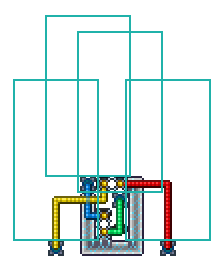
\includegraphics{images/254.png}
}
\end{center}
\caption{玩家试图左右移动时会触发玩家感应器并实化半砖将玩家推回;试图上平台时平台虚化,玩家掉落;试图下平台时下方半砖实化将玩家推回。}
\label{i253:254}
\end{figure}

\subsection{刷怪感应器}
刷怪感应器应用于刷怪场和Boss战场中,用来检测各种敌怪生成。大多数敌怪都可以直接触发压力板,所以一般情况下压力板就可以用来做刷怪感应器。穿墙怪不会触发压力板,只能使用特殊方法处理。

一个勉强及格的方案是在玩家周围放置压力板,穿墙怪攻击玩家时,玩家被击退,触发压力板,从而敌怪被检测到。这个方案的缺点是明显的,但是暂时也没有更好的方法。

\section{显示器}
显示器从原理上分为分段显示器、密集矩阵显示器、稀疏矩阵显示器、像素盒显示器。

\subsection{分段显示器}
分段显示器,指根据显示需要,将显示界面分为若干部分分别控制的显示器。在显示器中有部分光源状态始终同步的情况下,将这些光源当作单个光源处理,即为一段。在十进制数显中我们将显示器分为了七段;在二进制数显中分为了两段;在\autoref{dianlujichu}的思考题中,将月相显示器的分段任务留给了读者。

分段之后就可以设计控制电路。\autoref{i42:43}和\autoref{i71}中展示了十进制数显的两种不同控制电路风格。前者逻辑门排列紧密,需要更多排换线器;后者逻辑门有间隔,需要换线器更少但是占用空间更大。由于显示部分本身体积就很小,使用占用空间大的控制电路容易导致接线难看(\autoref{i113:114})。

另外,\autoref{i42:43}和\autoref{i71}展示了十进制数显的两种不同分段方式。一个分段显示器可以有很多种分段方式,不同的分段方式对应不同的控制电路和接线。一个自然的问题是,是否可以设计出一个分段方式使得控制电路最简?答案是,没有一个固定的套路可以使控制电路最简。尽管如此,我们往往还是可以做出部分简化。下面以一个例子来介绍优化分段方式的方法。

我们希望修改十进制数显的分段来减少控制电路的大小。数显初始分段如\autoref{i34:35}所示。在这个分段下,数字与分段的对应关系如\autoref{sjzsxctjxdxsjz}。

\begin{table}[!ht]
\centering
\begin{tabular}{c|ccccccc}
&a&b&c&d&e&f&g\\\hline
0&1&1&1&0&1&1&1\\
1&0&0&1&0&0&1&0\\
2&1&0&1&1&1&0&1\\
3&1&0&1&1&0&1&1\\
4&0&1&1&1&0&1&0\\
5&1&1&0&1&0&1&1\\
6&1&1&0&1&1&1&1\\
7&1&0&1&0&0&1&0\\
8&1&1&1&1&1&1&1\\
9&1&1&1&1&0&1&1
\end{tabular}
\caption{十进制数显传统接线的显示矩阵}\label{sjzsxctjxdxsjz}
\end{table}

上面的矩阵在$\mathbb{F}_2$\footnote{域$\mathbb{F}_2$包含0,1两个元素,可以将0看作偶数,1看作奇数。加法规则:0+0=1+1=0,0+1=1+0=1;乘法规则:0*0=0*1=1*0=0,1*1=1。}下的秩为7\footnote{后文中会介绍该矩阵的初等列变换操作并证明矩阵的列秩为7。},所以显示器至少要分成7段,没有办法减少段数。那么就没有可能减少控制电路中的换线器数量了吗?有的。在某些情况下,可以将同色的两段线连接到同一排换线器上并且使其不重叠(\autoref{})。用这种方法,7段线至多可以合并三对,这样就可以接在一行中。

我们对对应矩阵进行初等列变换,尝试将两列中的1分离。每列的列标是集合\{a, b, c, d, e, f, g\}的子集,列标为X的列的内容称为列X。初等列变换分为两种操作:
\begin{enumerate}
\item 交换列X和列Y,同时交换X和Y;
\item 将列X加到列Y上($\mathbb{F}_2$加法),同时将X改为X和Y的对称差\footnote{集合A与集合B的对称差定义为$A\triangle B=(A\cup B)-(A\cap B)$}。
\end{enumerate}

初等列变换过程如\autoref{bianhuanp1}和\autoref{bianhuanp2}。\autoref{bianhuanp1}使靠右的列的上部为0,经过这一步可以看出来矩阵的列秩为7;\autoref{bianhuanp2}使靠左的列的下部为0。经过变换后,第1列可以和第5列合并,第2列可以和第6列合并,第3列可以和第7列合并。合并后接线如\autoref{},注意由于合并的两列有重复段,在显示屏上不能使用同色电线,必须要使用额外的换线器。继续使用初等列变换可以减少换线器使用(\autoref{})。

\begin{figure}[p]
\centering
\subfloat[原矩阵]{
\label{bianhuan1}
\begin{tabular}{|c|ccccccc|}
&a&b&c&d&e&f&g\\\hline
0&1&1&1&0&1&1&1\\
1&0&0&1&0&0&1&0\\
2&1&0&1&1&1&0&1\\
3&1&0&1&1&0&1&1\\
4&0&1&1&1&0&1&0\\
5&1&1&0&1&0&1&1\\
6&1&1&0&1&1&1&1\\
7&1&0&1&0&0&1&0\\
8&1&1&1&1&1&1&1\\
9&1&1&1&1&0&1&1
\end{tabular}
}
\quad
\subfloat[将第1列加到第2,3,5,6,7列,交换第2,3列]{
\label{bianhuan2}
\begin{tabular}{|c|ccccccc|}
&abcefg&c&b&d&e&f&g\\\hline
0&1&0&0&0&0&0&0\\
1&0&1&0&0&0&1&0\\
2&1&0&1&1&0&1&0\\
3&1&0&1&1&1&0&0\\
4&0&1&1&1&0&1&0\\
5&1&1&0&1&1&0&0\\
6&1&1&0&1&0&0&0\\
7&1&0&1&0&1&0&1\\
8&1&0&0&1&0&0&0\\
9&1&0&0&1&1&0&0
\end{tabular}
}
\quad
\subfloat[将第2列加到第6列]{
\label{bianhuan3}
\begin{tabular}{|c|ccccccc|}
&abcefg&cf&b&d&e&f&g\\\hline
0&1&0&0&0&0&0&0\\
1&0&1&0&0&0&0&0\\
2&1&0&1&1&0&1&0\\
3&1&0&1&1&1&0&0\\
4&0&1&1&1&0&0&0\\
5&1&1&0&1&1&1&0\\
6&1&1&0&1&0&1&0\\
7&1&0&1&0&1&0&1\\
8&1&0&0&1&0&0&0\\
9&1&0&0&1&1&0&0
\end{tabular}
}
\quad
\subfloat[将第3列加到第4,6列,交换第4,5列]{
\label{bianhuan4}
\begin{tabular}{|c|ccccccc|}
&abcefg&cf&bdf&e&d&f&g\\\hline
0&1&0&0&0&0&0&0\\
1&0&1&0&0&0&0&0\\
2&1&0&1&0&0&0&0\\
3&1&0&1&1&0&1&0\\
4&0&1&1&0&0&1&0\\
5&1&1&0&1&1&1&0\\
6&1&1&0&0&1&1&0\\
7&1&0&1&1&1&1&1\\
8&1&0&0&0&1&0&0\\
9&1&0&0&1&1&0&0
\end{tabular}
}
\quad
\subfloat[将第4列加到第6列,交换第5,6列]{
\label{bianhuan5}
\begin{tabular}{|c|ccccccc|}
&abcefg&cf&bdf&ef&f&d&g\\\hline
0&1&0&0&0&0&0&0\\
1&0&1&0&0&0&0&0\\
2&1&0&1&0&0&0&0\\
3&1&0&1&1&0&0&0\\
4&0&1&1&0&1&0&0\\
5&1&1&0&1&0&1&0\\
6&1&1&0&0&1&1&0\\
7&1&0&1&1&0&1&1\\
8&1&0&0&0&0&1&0\\
9&1&0&0&1&1&1&0
\end{tabular}
}
\caption{}
\label{bianhuanp1}
\end{figure}

\begin{figure}[p]
\centering
\subfloat[将第6列加到第1,4,5列]{
\label{bianhuan6}
\begin{tabular}{|c|ccccccc|}
&abcefg&cf&bdf&ef&f&abcdfg&g\\\hline
0&1&0&0&0&0&0&0\\
1&0&1&0&0&0&0&0\\
2&1&0&1&0&0&0&0\\
3&1&0&1&1&0&0&0\\
4&0&1&1&0&1&0&0\\
5&0&1&0&0&1&1&0\\
6&0&1&0&1&0&1&0\\
7&0&0&1&0&1&1&1\\
8&0&0&0&1&1&1&0\\
9&0&0&0&0&0&1&0
\end{tabular}
}
\subfloat[将第5列加到第4列]{
\label{bianhuan7}
\begin{tabular}{|c|ccccccc|}
&abcefg&cf&bdf&ef&e&abcdfg&g\\\hline
0&1&0&0&0&0&0&0\\
1&0&1&0&0&0&0&0\\
2&1&0&1&0&0&0&0\\
3&1&0&1&1&0&0&0\\
4&0&1&1&1&1&0&0\\
5&0&1&0&1&1&1&0\\
6&0&1&0&1&0&1&0\\
7&0&0&1&1&1&1&1\\
8&0&0&0&0&1&1&0\\
9&0&0&0&0&0&1&0\\
\end{tabular}
}\\
\subfloat[将第7列加到第3,4,5,6列]{
\label{bianhuan8}
\begin{tabular}{|c|ccccccc|}
&abcefg&cf&bdf&ef&e&abcdfg&acf\\\hline
0&1&0&0&0&0&0&0\\
1&0&1&0&0&0&0&0\\
2&1&0&1&0&0&0&0\\
3&1&0&1&1&0&0&0\\
4&0&1&1&1&1&0&0\\
5&0&1&0&1&1&1&0\\
6&0&1&0&1&0&1&0\\
7&0&0&0&0&0&0&1\\
8&0&0&0&0&1&1&0\\
9&0&0&0&0&0&1&0
\end{tabular}
}
\subfloat[将第4列加到第2列]{
\label{bianhuan9}
\begin{tabular}{|c|ccccccc|}
&abcefg&cf&bdf&ce&e&abcdfg&acf\\\hline
0&1&0&0&0&0&0&0\\
1&0&1&0&0&0&0&0\\
2&1&0&1&0&0&0&0\\
3&1&1&1&1&0&0&0\\
4&0&0&1&1&1&0&0\\
5&0&0&0&1&1&1&0\\
6&0&0&0&1&0&1&0\\
7&0&0&0&0&0&0&1\\
8&0&0&0&0&1&1&0\\
9&0&0&0&0&0&1&0
\end{tabular}
}\\
\subfloat[将第2列加到第1列]{
\label{bianhuan10}
\begin{tabular}{|c|ccccccc|}
&abcefg&abeg&bdf&ce&e&abcdfg&acf\\\hline
0&1&0&0&0&0&0&0\\
1&1&1&0&0&0&0&0\\
2&1&0&1&0&0&0&0\\
3&0&1&1&1&0&0&0\\
4&0&0&1&1&1&0&0\\
5&0&0&0&1&1&1&0\\
6&0&0&0&1&0&1&0\\
7&0&0&0&0&0&0&1\\
8&0&0&0&0&1&1&0\\
9&0&0&0&0&0&1&0
\end{tabular}
}
\caption{}
\label{bianhuanp2}
\end{figure}

在上面的例子中,显示器在二进制输入为1010\~{}1111时会熄灭,也就是说显示器有十一种显示状态。如果我们不需要熄灭状态,减少一种状态,看看是否可以进一步减少换线器使用。

这里使用另一种技巧,我们先做一种预处理来减少矩阵中1的数量,这样有利于分离。定义矩阵列的反向操作:将该列列标的大小写互换,将该列01互换。标有大写的分段在接线时,其火把的01状态与正常情况相反。显然这个操作只有在初等列变换之前进行才有意义。

在初始的显示矩阵中,除了e列的1比0少,其他所有列的1都比0多,所以将其他所有列反向,可以减少矩阵中1的个数(\autoref{tab1})。对这个矩阵进行化简得到\autoref{},再作一些技巧上的处理(\autoref{}),就可以不使用换线器(\autoref{})。

\begin{table}[!ht]
\centering
\begin{tabular}{c|ccccccc}
&a&b&c&d&e&f&g\\\hline
0&0&0&0&1&1&0&0\\
1&1&1&0&1&0&0&1\\
2&0&1&0&0&1&1&0\\
3&0&1&0&0&0&0&0\\
4&1&0&0&0&0&0&1\\
5&0&0&1&0&0&0&0\\
6&0&0&1&0&1&0&0\\
7&0&1&0&1&0&0&1\\
8&0&0&0&0&1&0&0\\
9&0&0&0&0&0&0&0
\end{tabular}
\caption{}\label{tab1}
\end{table}

此外,还有一些方法可以作为化简手段:
\begin{itemize}
\item 交换矩阵的行。在之前的操作中,控制0\~{}9的十个逻辑门是按照数字顺序排列的。在减少可读性的情况下,可以改变它们的顺序,而改变它们的顺序可能会使矩阵的列分离开。因为顺序改变了,所以由递次电路控制的数显不能用这种方法。
\item 将某一段用两根线控制。7段线合并3对可以放在一行内,8段线合并4对也可以放在一行内。这样的话可以将显示矩阵中有较多1的一段分成有较少1的两段,可能有利于分离。
\item 将多于两段合并。这种方法的局限性较强,因为它影响多层控制电路的接线。如果最终可以只化为1层,那么这种方法可用。
\end{itemize}

\subsection{密集矩阵显示器}
用单色光源可以实现至少有一边长度至多为4的密集显示器(\autoref{i256:257})。

\begin{figure}[!ht]
\begin{center}
\subfloat{
\label{i256}

\includegraphics{images/256.png}
}
\qquad
\subfloat{
\label{i257}

\includegraphics{images/257.png}
}
\end{center}
\caption{第一行开关控制第一行火把,第二行开关控制第二行火把,第三行开关控制第三行火把,第四行开关控制第四行火把。}
\label{i256:257}
\end{figure}

用\nameref{sec21}可以实现任意尺寸的密集矩阵显示器。

\subsection{稀疏矩阵显示器}
稀疏矩阵显示器主要有两个参数:每个像素的光源面积与占用面积。稀疏矩阵显示器的大小不受限,一个典型的稀疏矩阵显示器如\autoref{i267:268}所示,当红线和蓝线在同一个逻辑帧输入时,火把响应,切换状态。显示器更新时,各行的红线逐次在各个逻辑帧激活,每列的蓝线在该逻辑帧选择性激活,用来控制该行的显示。这个例子中每个光源面积是4,占用面积是12,简称4占12,或4/12。目前使用这种显示器最杰出的作品是\url{https://www.bilibili.com/video/av22343683}。
\begin{figure}[!ht]
\centering

\includegraphics{images/267.png}
\qquad
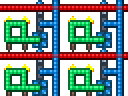
\includegraphics{images/268.png}
\caption{典型的矩阵显示器}
\label{i267:268}
\end{figure}

在这里我们看到控制每个像素的模块是一个占用3格的故障逻辑门。目前认为这是最小的控制单元\footnote{期待有人能开发出更小的显示器}。发光面积之间的间隔用来让控制的电线穿过。如果可以把火把摆在控制的电线上,那么就可以让显示器更紧凑(\autoref{i269:272})。
\begin{figure}[!ht]
\begin{center}
\subfloat[6/9]{
\label{i269:270}

\includegraphics{images/269.png}
\qquad
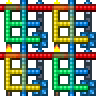
\includegraphics{images/270.png}
}
\qquad
\subfloat[1/4]{
\label{i271:272}

\includegraphics{images/271.png}
\qquad
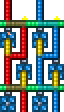
\includegraphics{images/272.png}
}
\end{center}
\caption{紧凑的矩阵显示器}
\label{i269:272}
\end{figure}

到这里你也许会有疑问,如果火把被摆在控制的电线上,不就会被控制的电线干扰吗?是的,是会被干扰,但是我们可以通过额外的激活来抵消这个干扰。具体说来,我们可以记录下每根控制电线激活的次数。如果一根控制电线激活了偶数次,那么它经过的火把是没有被干扰的。如果激活了奇数次,那么它经过的火把被取反,这时我们额外再激活一次这根线,就可以将火把恢复到没被干扰的状态。

接下来需要处理的一个问题是,额外激活的一次会不会干扰到某个像素?显然连接有效逻辑灯的电线不会,连接故障逻辑灯的电线可能会。事实上,如果我们先激活连接有效逻辑灯的电线,那么由于每根线都激活了偶数次,所有有效逻辑灯都会被关闭,此时再激活连接故障逻辑灯的电线不会干扰到任何一个像素。

此外,如果你足够细心,你会发现\autoref{i269:272}\subref{i271:272}中连接故障逻辑灯的电线也连接了有效逻辑灯,这不会出bug吗?在这种情况下,只要将有效逻辑灯的默认状态设为亮就行了。

还有一个非常巧妙的办法可以减少显示单元的面积,那就是使用小地图。半透明的小地图中每格2.5像素,在屏幕上是2像素和3像素交替排列。有很多使用小地图显示的例子:
\begin{itemize}
\item 【Terraria】做贪吃蛇—TheRedstoneCrafter \url{https://www.bilibili.com/video/av32265379}
\item 在Terraria中玩俄罗斯方块!? \url{https://www.bilibili.com/video/av38924330}
\end{itemize}

\section{自动化}

\begin{problemset}[思考题]
\item 为什么在分段显示器的化简中对矩阵进行初等列变换时需要对列标做对称差?
\item 为什么两边长都大于4的非像素盒密集矩形随机显示器不存在?
\end{problemset}